\section{Aplikacje WPF, MAUI i Dependency Injection w .NET}

\subsection{Wprowadzenie}
WPF (Windows Presentation Foundation) oraz .NET MAUI (Multi-platform App UI) są frameworkami do tworzenia aplikacji z interfejsem graficznym.  
\begin{itemize}
    \item \textbf{WPF} – przeznaczony dla systemu Windows, używa XAML i wzorca MVVM.  
    \item \textbf{.NET MAUI} – framework wieloplatformowy (Windows, Android, iOS, macOS), również oparty na XAML i MVVM.
\end{itemize}

\subsection{Struktura projektu WPF}
Projekt WPF składa się z plików:
\begin{itemize}
    \item \texttt{App.xaml} – deklaracja zasobów globalnych i punkt wejścia,
    \item \texttt{MainWindow.xaml} – główne okno aplikacji,
    \item \texttt{ViewModels/} – logika prezentacji,
    \item \texttt{Models/} – dane i logika biznesowa.
\end{itemize}

\begin{lstlisting}[language=XML, caption={Fragment App.xaml}]
<Application x:Class="WpfApp.App"
             xmlns="http://schemas.microsoft.com/winfx/2006/xaml/presentation"
             xmlns:x="http://schemas.microsoft.com/winfx/2006/xaml"
             StartupUri="MainWindow.xaml">
    <Application.Resources>
        <ResourceDictionary>
            <SolidColorBrush x:Key="PrimaryBrush" Color="#007ACC"/>
        </ResourceDictionary>
    </Application.Resources>
</Application>
\end{lstlisting}

\subsection{Struktura projektu MAUI}
Projekt MAUI ma podobny układ, ale rozszerzony o platformy:
\begin{itemize}
    \item \texttt{MauiProgram.cs} – główny punkt konfiguracji (DI, serwisy),
    \item \texttt{App.xaml} – konfiguracja wizualna aplikacji,
    \item \texttt{MainPage.xaml} – główny widok,
    \item katalogi: \texttt{Platforms/Android}, \texttt{Platforms/iOS}, \texttt{Platforms/Windows}.
\end{itemize}

\begin{lstlisting}[language=C, caption={Plik MauiProgram.cs}]
public static class MauiProgram
{
    public static MauiApp CreateMauiApp()
    {
        var builder = MauiApp.CreateBuilder();
        builder
            .UseMauiApp<App>()
            .ConfigureFonts(fonts =>
            {
                fonts.AddFont("OpenSans-Regular.ttf", "OpenSansRegular");
            });

        // Rejestracja serwisów
        builder.Services.AddSingleton<MainPageViewModel>();
        builder.Services.AddTransient<ApiService>();

        return builder.Build();
    }
}
\end{lstlisting}

\subsection{Dependency Injection (DI)}
\textbf{Dependency Injection} to wzorzec, który umożliwia wstrzykiwanie zależności zamiast ich tworzenia bezpośrednio w kodzie.  
Ułatwia testowanie i utrzymanie kodu, pozwalając wymieniać komponenty bez modyfikacji logiki aplikacji.

\begin{lstlisting}[language=C, caption={Przykład DI w WPF}]
public partial class MainWindow : Window
{
    private readonly IWeatherService _service;

    public MainWindow(IWeatherService service)
    {
        InitializeComponent();
        _service = service;
        DataContext = new MainViewModel(service);
    }
}
\end{lstlisting}

\begin{lstlisting}[language=C, caption={Rejestracja serwisów w konfiguracji}]
services.AddSingleton<IWeatherService, WeatherService>();
services.AddTransient<MainViewModel>();
\end{lstlisting}

\subsection{Zalety DI}
\begin{itemize}
    \item Redukuje sprzężenie między klasami,
    \item Umożliwia łatwe testowanie jednostkowe,
    \item Ułatwia utrzymanie i rozwój aplikacji,
    \item Pozwala dynamicznie wymieniać implementacje interfejsów.
\end{itemize}

\subsection{Cykl życia aplikacji MAUI}
W MAUI aplikacja przechodzi przez kilka etapów cyklu życia:
\begin{itemize}
    \item \texttt{OnStart()} – uruchomienie aplikacji,
    \item \texttt{OnSleep()} – uśpienie (np. minimalizacja),
    \item \texttt{OnResume()} – wznowienie działania.
\end{itemize}

\begin{lstlisting}[language=C, caption={Cykl życia aplikacji w MAUI}]
protected override void OnStart()
{
    Console.WriteLine("Aplikacja wystartowała");
}

protected override void OnSleep()
{
    Console.WriteLine("Aplikacja uśpiona");
}

protected override void OnResume()
{
    Console.WriteLine("Aplikacja wznowiona");
}
\end{lstlisting}

\subsection{Diagram cyklu życia aplikacji MAUI}
\begin{center}
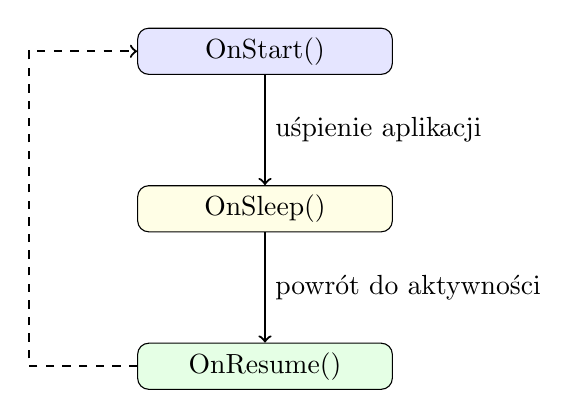
\begin{tikzpicture}[node distance=2cm, every node/.style={align=center}]
\node (start) [draw, rounded corners, fill=blue!10, text width=3cm] {OnStart()};
\node (sleep) [draw, rounded corners, fill=yellow!10, below of=start, text width=3cm] {OnSleep()};
\node (resume) [draw, rounded corners, fill=green!10, below of=sleep, text width=3cm] {OnResume()};

\draw[->, thick] (start) -- node[right]{uśpienie aplikacji} (sleep);
\draw[->, thick] (sleep) -- node[right]{powrót do aktywności} (resume);
\draw[->, thick, dashed] (resume) -- ++(-3,0) |- (start);
\end{tikzpicture}
\end{center}

\subsection{Tworzenie usług i integracja z API}
Aplikacje WPF i MAUI często komunikują się z API REST poprzez serwisy.

\begin{lstlisting}[language=C, caption={Przykład klasy serwisowej w MAUI}]
public class ApiService
{
    private readonly HttpClient _client = new();

    public async Task<List<CityDto>> GetCitiesAsync()
    {
        var response = await _client.GetAsync("https://localhost:7294/api/cities");
        response.EnsureSuccessStatusCode();
        var json = await response.Content.ReadAsStringAsync();
        return JsonSerializer.Deserialize<List<CityDto>>(json)!;
    }
}
\end{lstlisting}

\begin{lstlisting}[language=C, caption={Przykład użycia serwisu w ViewModelu}]
public class CitiesViewModel : INotifyPropertyChanged
{
    private readonly ApiService _api;
    public ObservableCollection<CityDto> Cities { get; set; } = new();

    public CitiesViewModel(ApiService api)
    {
        _api = api;
        LoadCitiesCommand = new RelayCommand(async () => await LoadCities());
    }

    public ICommand LoadCitiesCommand { get; }

    private async Task LoadCities()
    {
        var result = await _api.GetCitiesAsync();
        Cities.Clear();
        foreach (var c in result)
            Cities.Add(c);
    }

    public event PropertyChangedEventHandler? PropertyChanged;
}
\end{lstlisting}

\subsection{Powiązanie z interfejsem w MAUI}
\begin{lstlisting}[language=XML, caption={Fragment MainPage.xaml}]
<ContentPage xmlns="http://schemas.microsoft.com/dotnet/2021/maui"
             xmlns:x="http://schemas.microsoft.com/winfx/2009/xaml"
             xmlns:vm="clr-namespace:MauiApp.ViewModels"
             x:Class="MauiApp.MainPage">

    <ContentPage.BindingContext>
        <vm:CitiesViewModel />
    </ContentPage.BindingContext>

    <CollectionView ItemsSource="{Binding Cities}">
        <CollectionView.ItemTemplate>
            <DataTemplate>
                <StackLayout Padding="10">
                    <Label Text="{Binding Name}" FontSize="18"/>
                    <Label Text="{Binding Population}" FontSize="14" TextColor="Gray"/>
                </StackLayout>
            </DataTemplate>
        </CollectionView.ItemTemplate>
    </CollectionView>

    <Button Text="Załaduj miasta" Command="{Binding LoadCitiesCommand}" />
</ContentPage>
\end{lstlisting}

\subsection{MAUI Shell Navigation}
Shell to zaawansowany system nawigacji w .NET MAUI, obsługujący routing, Flyout i TabBar.

\subsubsection{Rejestracja tras}
\begin{lstlisting}[language=C, caption={Rejestracja route w AppShell.xaml.cs}]
	public AppShell()
	{
		InitializeComponent();
		
		// Rejestracja tras
		Routing.RegisterRoute("details", typeof(DetailsPage));
		Routing.RegisterRoute("edit", typeof(EditPage));
	}
\end{lstlisting}

\subsubsection{Nawigacja z parametrami}
\begin{lstlisting}[language=C, caption={Nawigacja do strony szczegółów}]
	// W ViewModelu lub code-behind
	await Shell.Current.GoToAsync("details", new Dictionary<string, object>
	{
		{"Item", selectedItem},
		{"ItemId", selectedItem.Id}
	});
\end{lstlisting}

\subsubsection{Odbieranie parametrów}
\begin{lstlisting}[language=C, caption={Odbieranie parametru w DetailsPage}]
	[QueryProperty(nameof(Item), "Item")]
	[QueryProperty(nameof(ItemId), "ItemId")]
	public partial class DetailsPage : ContentPage
	{
		public Item Item { get; set; }
		public int ItemId { get; set; }
		
		protected override void OnAppearing()
		{
			base.OnAppearing();
			Console.WriteLine($"Otrzymano Item: {Item.Name}, ID: {ItemId}");
		}
	}
\end{lstlisting}

\subsubsection{Shell Flyout i TabBar}
\begin{lstlisting}[language=XML, caption={Przykład Shell z Flyout}]
	<Shell xmlns="http://schemas.microsoft.com/dotnet/2021/maui"
	x:Class="MyApp.AppShell">
	
	<FlyoutItem Title="Home" Icon="home.png">
	<ShellContent Route="home" ContentTemplate="{DataTemplate local:HomePage}" />
	</FlyoutItem>
	
	<FlyoutItem Title="Settings" Icon="settings.png">
	<ShellContent Route="settings" ContentTemplate="{DataTemplate local:SettingsPage}" />
	</FlyoutItem>
	
	<TabBar>
	<Tab Title="Browse" Icon="browse.png">
	<ShellContent Route="browse" ContentTemplate="{DataTemplate local:BrowsePage}" />
	</Tab>
	<Tab Title="Profile" Icon="profile.png">
	<ShellContent Route="profile" ContentTemplate="{DataTemplate local:ProfilePage}" />
	</Tab>
	</TabBar>
	</Shell>
\end{lstlisting}

\subsection{MAUI Essentials -- dostęp do funkcji platformy}
MAUI Essentials to zestaw API zapewniających dostęp do funkcji urządzeń (geolokalizacja, czujniki, kamera, itp.).

\subsubsection{Connectivity -- sprawdzanie połączenia}
\begin{lstlisting}[language=C, caption={Sprawdzanie dostępu do Internetu}]
	var networkAccess = Connectivity.Current.NetworkAccess;
	if (networkAccess == NetworkAccess.Internet)
	{
		Console.WriteLine("Połączenie z Internetem dostępne");
	}
	else
	{
		Console.WriteLine("Brak połączenia");
	}
	
	// Nasłuchiwanie zmian
	Connectivity.Current.ConnectivityChanged += (sender, args) =>
	{
		Console.WriteLine($"Zmiana połączenia: {args.NetworkAccess}");
	};
\end{lstlisting}

\subsubsection{Geolocation -- lokalizacja}
\begin{lstlisting}[language=C, caption={Pobieranie lokalizacji GPS}]
	try
	{
		var location = await Geolocation.GetLocationAsync(new GeolocationRequest
		{
			DesiredAccuracy = GeolocationAccuracy.Medium,
			Timeout = TimeSpan.FromSeconds(10)
		});
		
		if (location != null)
		{
			Console.WriteLine($"Lat: {location.Latitude}, Lon: {location.Longitude}");
		}
	}
	catch (FeatureNotSupportedException)
	{
		Console.WriteLine("Geolokalizacja nie jest wspierana na tym urządzeniu");
	}
	catch (PermissionException)
	{
		Console.WriteLine("Brak uprawnień do lokalizacji");
	}
\end{lstlisting}

\subsubsection{DeviceInfo -- informacje o urządzeniu}
\begin{lstlisting}[language=C, caption={Informacje o urządzeniu}]
	Console.WriteLine($"Model: {DeviceInfo.Model}");
	Console.WriteLine($"Producent: {DeviceInfo.Manufacturer}");
	Console.WriteLine($"Platforma: {DeviceInfo.Platform}");
	Console.WriteLine($"Wersja: {DeviceInfo.VersionString}");
	Console.WriteLine($"Typ: {DeviceInfo.Idiom}"); // Phone, Tablet, Desktop, TV
\end{lstlisting}

\subsection{Kompilacja warunkowa -- kod specyficzny dla platformy}
W MAUI można pisać kod specyficzny dla danej platformy przy użyciu dyrektyw preprocesora.

\begin{lstlisting}[language=C, caption={Kod warunkowy dla Android i iOS}]
	public void ShowNativeAlert()
	{
		#if ANDROID
		Android.Widget.Toast.MakeText(
		Android.App.Application.Context, 
		"To jest Android", 
		Android.Widget.ToastLength.Short
		).Show();
		#elif IOS
		var alert = UIKit.UIAlertController.Create(
		"Informacja", 
		"To jest iOS", 
		UIKit.UIAlertControllerStyle.Alert
		);
		alert.AddAction(UIKit.UIAlertAction.Create("OK", UIKit.UIAlertActionStyle.Default, null));
		// Wyświetl alert
		#elif WINDOWS
		System.Diagnostics.Debug.WriteLine("To jest Windows");
		#endif
	}
\end{lstlisting}

\textbf{Dostępne dyrektywy:}
\begin{itemize}
	\item \texttt{\#if ANDROID} -- kod tylko dla Android,
	\item \texttt{\#if IOS} -- kod tylko dla iOS,
	\item \texttt{\#if WINDOWS} -- kod tylko dla Windows,
	\item \texttt{\#if MACCATALYST} -- kod dla macOS (Catalyst).
\end{itemize}

\subsection{Różnice WPF vs MAUI -- rozszerzone}
\begin{center}
	\begin{tabular}{|p{3.5cm}|p{5cm}|p{5cm}|}
		\hline
		\textbf{Cecha} & \textbf{WPF} & \textbf{MAUI} \\
		\hline
		Platformy & Tylko Windows & Android, iOS, Windows, macOS \\
		\hline
		Projekt & Klasyczny (.csproj) & Single Project \\
		\hline
		Customizacja UI & Dependency Properties & Handlers \\
		\hline
		Dostęp do natywnych API & Ograniczony (P/Invoke) & MAUI Essentials + kod warunkowy \\
		\hline
		Lifecycle & OnStartup, OnExit & OnStart, OnSleep, OnResume \\
		\hline
		Hot Reload & Desktopowy & Wieloplatformowy (emulatory + urządzenia) \\
		\hline
		Uprawnienia & Nie wymagane & Wymagane (kamera, lokalizacja, etc.) \\
		\hline
	\end{tabular}
\end{center}

\subsection{Podsumowanie rozdziału}
\begin{itemize}
    \item WPF i MAUI używają XAML i wzorca MVVM.
    \item Dependency Injection umożliwia niezależność komponentów.
    \item Cykl życia aplikacji MAUI obejmuje start, uśpienie i wznowienie.
    \item Serwisy wstrzykuje się do ViewModeli i komunikują z API.
\end{itemize}

\subsection{Pytania kontrolne}
\begin{enumerate}
    \item Jakie są główne różnice między WPF a .NET MAUI?
    \item Do czego służy plik \texttt{MauiProgram.cs}?
    \item Jak działa Dependency Injection i jakie ma zalety?
    \item Jak wygląda cykl życia aplikacji w MAUI?
    \item Jak ViewModel komunikuje się z serwisem API?
\end{enumerate}
